% --------------------
% Layout and standard configuration
% --------------------
\documentclass[a4paper,11pt]{article} 

\usepackage[applemac]{inputenc}
\usepackage[english]{babel}			% alternativ: \usepackage{ngerman} oder bei babel: ngerman
\usepackage[T1]{fontenc} 				% (Trennung von W�rtern, die Umlaute enthalten) 
\usepackage[bottom,stable,multiple,hang]{footmisc} 		% Fussnoten / Optionen: hang (d.h. ohne Einr�cken)

\usepackage{setspace} 							% Zeilenabstand - moderieren durch: \setstretch{1.2}
\usepackage{ragged2e}
	% The pack?age de?fines new com?mands 
	% \Cen?ter?ing, \RaggedLeft, \RaggedRight and new en?vi?ron?ments Cen?ter, FlushLeft, and FlushRight
	% \justifying switches back to justified text after ragged text has been switched on.


% -----------------------------------------------------------------------------------------------------------------------
% Layout of Text
% -----------------------------------------------------------------------------------------------------------------------	
\usepackage{multicol}
		% use \usepackage{wrapfig} and \usepackage{wraptable}	 for inside - tables and figures
		% usage: 
		% \begin{multicols}{3} 			% unbalanced: \begin{multicols*}{3} 
			% [
			% \section{First Section}
			% THIS IS NOT PART OF THE COLUMNS
			% ]
			% THIS IS INSIDE COLUMS
			% \end{multicols}	
		% \columnbreak 				% go to next column			
	\setlength{\columnsep}{1.5pc}
		% \setlength{\columnseprule}{0.7pt}
		% \def\columnseprulecolor{\color{blue}}	
	\setcounter{columnbadness}{7000}
	\setcounter{finalcolumnbadness}{7000}	

\usepackage[neverdecrease]{paralist}		% for compactitem
	% neverdecrease: If the width of the labels is adjusted, this option avoids the decrease of the width
	\setlength{\pltopsep}{-\topsep}			% Space between first item and preceding paragraph.
	\setlength{\plpartopsep}{-\plpartopsep} 	% Extra space added to \topsep when environment starts a new paragraph
	%\plitemsep							% Space between successive items.
	%\plparsep 							% Space between paragraphs within an item � the \parskip for this environment.
		% usage: {inparaenum, asparaenum, asparaitem, inparaitem, compactenum, compactitem}
			%	\begin{inparaenum}
			%	\item LIONS, ; 
			%	\item DRAGONS, and finally
			% 	\item MONSTERS
			%	\end{inparaenum}				

						

% -----------------------------------------------------------------------------------------------------------------------
% Margins
% -----------------------------------------------------------------------------------------------------------------------
\usepackage[]{geometry} %
\topmargin -22mm 				% Margin at top of page above all printing
\headheight 14mm 				% Height of the header (appears atop all pages)
\headsep 12mm 				% Distance from bottom of header to the body of text on a page.
\topskip 5mm 					% Distance from top of main text box to the baseline of the first line of text in the main text box.
	
\textheight 255mm
\textwidth 157mm
\footskip 15mm
\oddsidemargin -8mm 			% Left margin on odd numbered pages
\evensidemargin -8mm

\marginparsep 3mm
\marginparwidth 20mm 

\parskip 0.6em					% Distance between paragraphs. %vorher 0.7
\parindent	 0pt 					% Amount of indentation at the first line of a paragraph. % 7mm oder \noindent


\clubpenalty = 9000 				% Disable single lines at the start of a paragraph (Schusterjungen) / 10000 maximaler Wert!
\widowpenalty = 9000 
\displaywidowpenalty = 9000		% Disable single lines at the end of a paragraph (Hurenkinder) / 10000 maximaler Wert!	
% -----------------------------------------------------------------------------------------------------------------------
% -----------------------------------------------------------------------------------------------------------------------



% -----------------------------------------------------------------------------------------------------------------------
% Signs and Symbols, Math ||�Graphics and Colors
% -----------------------------------------------------------------------------------------------------------------------
\usepackage{amsmath}
\usepackage{amssymb}
\usepackage{amsthm}
\usepackage{stmaryrd}
\usepackage{array}
\usepackage{ifsym}
\usepackage{wasysym}
\usepackage{units}

\usepackage{pdfpages}
\usepackage{graphics}
\usepackage{graphicx}
\usepackage{epsfig}
\usepackage{calc} 		% for making internal calculations...

% ----------------------------------------------------
\graphicspath{{pix/}}         						% Festlegung des Pfades zu den Bildern

\usepackage{color}
\usepackage{colorsapplemac}					% Apple-Farben, defined by Felix 
										% English and German
%\usepackage{latexcolor}						% full color set from http://latexcolor.com/
%\usepackage{ocol}						% full color set from http://latexcolor.com/
										
% \usepackage[usenames,dvipsnames,svgnames,table]{xcolor}
% \usepackage{forest}						% For drawing linguistic trees

\usepackage{xspace}	% f�r Leerzeichen hinter W�rtern / usefuls for macros!
	% \xspaceaddexceptions{\fvscitealp \fvcitealp \fscitealp \fcitealp} 
	% Ausnahmen, dass vor Fussnoten kein Leerzeichen ist, hilfreich bei mehreren Fussnoten
% -----------------------------------------------------------------------------------------------------------------------
% -----------------------------------------------------------------------------------------------------------------------


% -----------------------------------------------------------------------------------------------------------------------
% Inserting Graphics & Pictures |� and Captions
% -----------------------------------------------------------------------------------------------------------------------
\usepackage{subfig}				% subfigures
\usepackage{wrapfig}			% to create wrap figures within text
\usepackage[export]{adjustbox}		% to align figures
\usepackage{pdflscape}			% support to the environment landscape of package lscape by setting the PDF page attribute /Rotate

\usepackage[labelfont={sf,bf}]{caption}
	% 	\usepackage[figurename=Figure,tablename=Table,listfigurename= List of Figures,listtablename= List of Tables]{caption}
	% 	\DeclareCaptionFont{captionfarbe}{\color{\captionfarbe}}
	% 	\captionsetup{labelsep=colon-newline}
	% 	\captionsetup{textfont={captionfarbe,sl}}
	% 	\DeclareCaptionLabelSeparator{period-newline}{. \\}
	% 	justification=raggedright % textfont={it}
	
\usepackage[]{sidecap} 
	% 	Options:
	%		margincaption 
	% 		innerbody, outerbody, centerbody, leftbody oder rightbody
	% 	\captionsetup{labelsep=colon-newline}
	% 	\captionsetup{textfont={captionfarbe,sl}}
	% 	\renewcommand\sidecaptionsep{} %default ist \marginparsep 

\usepackage{fpic2}	
	% May require packages {caption, sidecap}
\newcommand{\fpicframe}{0.3mm}
\newcommand{\fpicframedistance}{2mm}
\newcommand{\fpicwidth}{\textwidth-\fpicframedistance-\fpicframedistance-\fpicframe-\fpicframe}
	% Standard options for inserting a picture / define for fpic2-Package: 
	



% ----------------------?!?!?--------------------------?!?!?---------------------------!??!?!--------------------------------------------
% F�r ein Bild:
% \fpicw{adresse}{\fpicwidth}{caption}{Labelfuerref}{captionfuertableofcontents}{platzierungdefault_tbp}
% Requires the package 	fpic2.sty


%  \fpicw{adresse}{\fpicwidth}{caption}{Labelfuerref}{captionfuertableofcontents}{tbp}
 	% Abbildung mit Sidecap-Bildunterschrift und vorher im Header definierten Rahmen, etc.
	% aus dem Packet: fpicx.sty

%  \fpicempty{inhalt}{nix}{caption}{Labelfuerref}{captionfuertableofcontents}{tbp}
 	% Abbildung mit Sidecap-Bildunterschrift und vorher im Header definierten Rahmen, etc.
	% aus dem Packet: fpicx.sty
% ----------------------?!?!?--------------------------?!?!?---------------------------!??!?!--------------------------------------------







% -----------------------------------------------------------------------------------------------------------------------
% Prettyref - f�r Querverweise:
% --------------------
\usepackage{prettyref}
% \newrefformat{pr�fix}{code}	% \titleref{} oder \currenttitle{}
	\newrefformat{fig}{figure~\ref{#1}}
	\newrefformat{tab}{table~\ref{#1}}
	\newrefformat{sec}{section~\ref{#1}}
	\newrefformat{ssec}{subsection~\ref{#1}}
	\newrefformat{foo}{footnote~\ref{#1}}
	\newrefformat{app}{appendix~\ref{#1}}
	
	% usage:			\label{tab:1}
	% access via: 		\prettyref{tab:1} 
	% 				\pageref{tab:1}  
	% 				\ref{tab:1}
% -----------------------------------------------------------------------------------------------------------------------




% -----------------------------------------------------------------------------------------------------------------------
% Literature and Biblatex
% -----------------------------------------------------------------------------------------------------------------------

\usepackage[backend=bibtex, style=authoryear, natbib, doi=false, isbn=false, url=false]{biblatex}
\usepackage{url}						% intended for email addresses, hypertext links, directories/paths
\usepackage{citejournal, citettl}				% Package by Felix to Cite the JOURNAL / title
									% Usage: \citejournal{REFERENCE}

% Options: 
% isbn=false will suppress any isbn fields included in your .bib file. (It works the same way for url, doi and eprint.) (Introduced in v0.9)
% firstinits=true will render all first and middle names as initials. (Introduced in v0.8)
% dashed=false (available for the authoryear, authortitle, and verbose bibliography styles) will print recurring author/editor names instead of replacing them by a dash. (Introduced in v0.9)

% Styles: 			style=apa, style=authoryear, 
% Citestyle: 		citestyle=authoryear 

%\AtBeginBibliography{\footnotesize}		% Small font in Bibliography
\bibliography{%
	/Users/loro/Documents/Documents/00_science/00_bibdesk/00-0_sosi/000_SocialSciences_Bibdesk_FME.bib,%
	}
% -----------------------------------------------------------------------------------------------------------------------
% -----------------------------------------------------------------------------------------------------------------------


% -----------------------------------------------------------------------------------------------------------------------
% Boxes and HighLIGHTING
% -----------------------------------------------------------------------------------------------------------------------
\usepackage{fboxes}		% Package by Felix for boxes
					% Usage: 
					% \boxx{width}{FRthickness}{FRdistance}{colorTXT}{colorBACKG}{refLABEL}{TXT}
					% \boxx{\textwidth-4.8mm}{0.4mm}{2mm}{zinn}{schnee}{label}{TEXT}
					% Define a new boxxx-Class:
					 \newcommand{\boxxx}[1]{\boxx{\textwidth-4.8mm}{0.4mm}{2mm}{zinn}{schnee}{}{#1}}
					%\boxxx{TEXT}
					% very simple box: 
					% \fbox{\parbox[b]{\textwidth}{txt}} 

% Highlight!
% --------------------
\usepackage{soul} 
\sethlcolor{lightblue}		% honeydew, lemon, ... 
	% 	\hl{TEXT}		zum Highlighten
						
% -----------------------------------------------------------------------------------------------------------------------
% -----------------------------------------------------------------------------------------------------------------------



% -----------------------------------------------------------------------------------------------------------------------
% Headers & Footers
% --------------------

\usepackage{fancyhdr}
	\pagestyle{fancy}
		
	\fancyheadoffset[LE,RO]{\marginparsep+\marginparwidth}
	\fancyfootoffset[LE,RO]{\marginparsep+\marginparwidth}
		
	\renewcommand{\sectionmark}[1]{\markboth{#1}{}} 
		% \renewcommand{\subsectionmark}[1]{\markright{#1}} % markright als subsection

	% header
	\fancyhf{} 		% clears the header and footer, otherwise the elements of the default "plain" page style will appear.
	\lhead{}		%\thesection \leftmark} 	
	\chead{}
	\rhead{\thepage} 			
	\renewcommand{\headrulewidth}{0.3pt}
	
	% footer
	\rfoot{}
	\cfoot{} 			% \thepage
	\lfoot{}
	% \renewcommand{\footrulewidth}{0.6pt}
	
	% 	\cfoot{\thepage\ of \pageref{LastPage}}		% requires \usepackage{lastpage} and \usepackage{ifthen}
	%	\thesection		% adds number of the current section.
	%	\leftmark			% adds name and number of the current top-level structure
	%	\rightmark			% adds name and number of the current next to top-level structure
	%	\fancyhf{} 			% clears the header and footer, otherwise the elements of the default "plain" page style will appear.
	
	% For  double-sided documents
	%	\fancyhead[LE,RO]{Share\LaTeX}					% E - even, O - odd, L R C
	%	\fancyhead[RE,LO]{Guides and tutorials}
	%	\fancyfoot[CE,CO]{\leftmark}
	%	\fancyfoot[LE,RO]{\thepage}

	
% -----------------------------------------------------------------------------------------------------------------------
% -----------------------------------------------------------------------------------------------------------------------




% -----------------------------------------------------------------------------------------------------------------------
% Hyperref - hyper references, etc.
% -----------------------------------------------------------------------------------------------------------------------
% requieres packages{colors_applemac}
% see all options at: 			http://mirror.switch.ch/ftp/mirror/tex/macros/latex/contrib/hyperref/doc/options.pdf
	% DELETE THIS LINE after it works: 
	%\usepackage[pdftex, hidelinks , plainpages=false, pdfpagelabels, breaklinks, pagebackref=false]{hyperref} 

\usepackage[pdftex]{hyperref}

\hypersetup{
	unicode=false,          			% non-Latin characters in Acrobat�s bookmarks
	pdftoolbar=false,        		% show Acrobat�s toolbar?
	pdfmenubar=false,        		% show Acrobat�s menu?
	pdffitwindow=true,     		% window fit to page when opened
	pdfstartview={FitH},    		% {FitB, FitH, Fit} fits the width of the page to the window
	bookmarksopenlevel=2 		% wie weit das Inhaltsverzeichnis schon ge�ffnet sein soll
    	pdfnewwindow=true,      		% links in new window
	pdfpagemode= UseThumbs, 	% {FullScreen, UseNone, UseThumbs, None, UseOutlines, FullScreen, UseOC, UseAttachments}
}

	% Further usage:
	% ???\href{options}{URL}{text}
			% options: {page=1} page# of remote PDF, {pdfremotestartview}, {pdfnewwindow}
	% \hyperlink{name}{text}	-> linking to \hypertarget{name}{text}						
	% \urlstyle{same}	% URLs in same style as text	
	
\usepackage[all]{hypcap} 
% Since hyperref points to the caption created within the float environment, which is always set below a figure or table, the figure or table itself will not be visible[3]. A workaround exists by using the package


% -----------------------------------------------------------------------------------------------------------------------
% -----------------------------------------------------------------------------------------------------------------END
% -----------------------------------------------------------------------------------------------------------------------




% -----------------------------------------------------------------------------------------------------------------------
% Makros and Abbreviations
% -----------------------------------------------------------------------------------------------------------------------
\newcommand{\ca}{ca.\xspace}



% 
% TUTORIAL
% -----------------------------------------------------------------------------------------------------------------------
% Short commands to insert...
% -----------------------------------------------------------------------------------------------------------------------
	
	% Insert Picture!
	% \fpicw{adresse}{\fpicwidth}{caption}{Labelfuerref}{captionfuertableofcontents}{platzierungdefault_tbp}
	% Requires the package 	fpicx.sty


% -----------------------------------------------------------------------------------------------------------------------
% -----------------------------------------------------------------------------------------------------------------------
	



% -----------------------------------------------------------------------------------------------------------------------
% Listen und Tabellen
% --------------------
\usepackage{longtable}			% table spanning multiple pages
\usepackage{colortbl}			% colors in table
\usepackage{booktabs}	 		% nicer layout of tables {\toprule, \midrule, \bottomrule}
\usepackage{caption}			% \caption*  -- to create an unnumbered table float. 
\usepackage{multirow}			% \multirow{4}*{\minitab[c]{Common \\ multi text}} & Column TEXT\\


% -------------------------------------------------------------
% Rotating tables: 
\usepackage{tabularx}
\usepackage{rotating}			% f�r die turn-Umgebung
\usepackage{pdfpages}
\usepackage{relsize}				% f�r \smaller-Befehl

	\newcolumntype{L}[1]{>{\RaggedRight\arraybackslash}p{#1}}
	\newcolumntype{R}[1]{>{\RaggedLeft\arraybackslash}p{#1}}

	\newcolumntype{U}[1]{%
		>{\begin{turn}{90}\begin{minipage}{#1}%
			\scriptsize\raggedright\hspace{0pt}}l%
		<{\end{minipage}\end{turn}}%
	}

	\newcolumntype{K}[1]{%
		>{\begin{turn}{90}\begin{minipage}{#1}%
			\scriptsize\raggedright\hspace{0pt}}l%
		<{\end{minipage}\end{turn}}%
	}
	
	\newcolumntype{V}[1]{% 						% Spaltentyp f�r gest�rzten Tabellenkopf
		>{\begin{turn}{90}\begin{minipage}{#1}%
			\smaller\raggedright\hspace{0pt}}l% 		% \smaller: Schrift in Tabellenk�pfen
		<{\end{minipage}\end{turn}}% 				% einen Grad kleiner setzen
	}
	
	\newcolumntype{W}[2]{% zwei Parameter: #1 H�he, #2 Breite
	>{\begin{turn}{90}\begin{minipage}[][#2][c]{#1}%
	\smaller\raggedright\hspace{0pt}}l%
	<{\end{minipage}\end{turn}}%
	}
	% usage: 
		% see sq-rotate-table

% -----------------------------------------------------------------------------------------------------------------------
% -----------------------------------------------------------------------------------------------------------------------




% -----------------------------------------------------------------------------------------------------------------------
% all this: already in TXT-document
% -----------------------------------------------------------------------------------------------------------------------
%
%\begin{document}
%
%
%%-------------------------------
%%\title{___TITLE____}
%%\author{Felix Meissner\\University of Zurich}
%%\date{2014}
%%\maketitle
%% 	\setstretch{1.05}
%%	\pagenumbering{arabic}


%
%%-------------------------------

\hypersetup{
	%
	pdftitle={Adapt or Die: How Watching Others Can Help you to Perform Better},
  	pdfauthor={Felix Meissner},
  	%pdfsubject={\coverkind},
  	pdfkeywords={Social Learning, Individual Learning, Experiential Learning, Direct Learning, Learning from Experience, Multi-armed Bandit, Agent-Based Simulation},
  	pdfcreator={Felix Meissner},
    	%pdfproducer={},
	%
}

\begin{document}
\vspace{-2cm}
\nopagebreak
\vspace{-2cm}
\nopagebreak

% Hierarchy-guided learning
%\title{\vspace{-1.2cm}Combining Direct and Vicarious Learning Under Varying Levels of Heterogeneity and Change\vspace{-1cm}}
\title{\vspace{-1.2cm}Adapt or Die: \newline How Watching Others Can Help You to Perform Better\thanks{The author would like to thank Olivia and Stefano for both stimulating and directing the development of this working paper.}
}
\author{Felix Meissner, ETHZ and UZH\thanks{felix.meissner@business.uzh.ch}}
\date{11th of December 2015}

\maketitle
\setstretch{1.17}
\vspace{-0.7cm}

\thispagestyle{empty}

%\begin{abstract}
%Organizations complement experiential learning with vicarious learning in order to optimize their search processes. Watching other reference organizations that are solving similar problems can stimulate and direct an organization's own explorative activities. \newline
%We find that both complete and incomplete information about other organizations' choices and performance outcomes stimulates and directs firm-internal experimentation, thereby enhancing performance. Surprisingly, both in environments with high inter-organizational heterogeneity as well as in dynamic environments with high probabilities of turbulence, incomplete information can be even more effective in guiding search and increasing steady state performance. Further, steady state performance is higher under conditions of intermediate and high levels of turbulence if reference firms are less homogeneous.
%\end{abstract}


% ABSTRACT OF RESEARCH
\begin{abstract}
Organizations complement experiential learning with social learning in order to optimize their search processes. Watching the activities and performance of other reference organizations that are solving similar problems can stimulate and direct organizations' own explorative activities through heuristics that guide search.
With this research project, I aim at improving our understanding of the micro-mechanisms and interactions of direct and social learning from reference organizations in a firm's network. More specific, I investigate how varying degrees of social learning under varying degrees of similarity have an impact on organizational performance. Using a simulation that is based on a modification of the multi-armed bandit model I find the following: 

Organizations that complement individual learning with social learning can substantially improve their learning speed and performance in the short run. However, in the long run, organizations that rely too much on watching other organizations will get stuck on lower performance plateaus. This effect is strongly moderated by the heterogeneity among organizations: The more an organization differs from the peers it is watching, the less it can learn from them. 

%Both complete and incomplete information about other organizations' choices and performance outcomes stimulates and directs firm-internal exploration, thereby increasing performance in the long run. Interestingly, incomplete knowledge of reference organizations (a higher degree of bounded rationality) is more effective in guiding own search behavior for environments with intermediate and high levels of inter-organizational heterogeneity, resulting in higher levels of performance in the long run. 
%I further find that while the value of complete information erodes with increasing levels of inter-firm heterogeneity, the value of incomplete information slightly increases. Therefore, vicarious learning of organizations that are bounded rational benefits from a higher heterogeneity of the reference firms to guide own search activities. 
%Under conditions of turbulence (change affecting the performance of a firm's possible choices), vicarious learning can enable organizations to hold performance levels relatively constant, even for increasing probabilities of such turbulence shocks. Surprisingly, performance is higher under settings of intermediate and high levels of turbulence if reference firms are less homogeneous.
\end{abstract}

\pagebreak


\section*{Introduction}

% Interorganizational imitation of practices and structures plays a central role in several theories of organizational action. Theories of organizational learning, for example, argue that organizations copy other organizations, letting others absorb the costs of experimentation or discovery (Dutton and Freedman, 1985; Levitt and March, 1988; Lant and Mezias, 1990; Bolton, 1992). 

The study of organizational search and learning is an important and popular field in organizational theory and strategy research. Learning from search allows organizations to adapt to their environment, better respond to arising problems, take advantage of market opportunities, and increase their competitive advantage \citep{Argote2012_Organizational-Learning-Curves:-An-Overview, ArgoteTodorova2007_Organizational-Learning_IntRevOfIndustrialAndOrganizationalPsychology, Haunschild1993_Interorganizational-Imitation-The-Impact-of-Interlocks_ASQ, MarchSimon1958_Organizations}. To benefit from these opportunities, organizations invest in a variety of different learning activities and approaches \citep{BinghamDavis2012_Learning-Sequences-Their-Existence-Effect-and-Evolution_AMJ}. %Therefore, Organizations need to continuously balance exploitative and explorative activities to address organizational challenges and maximize the performance of their practices \citep{CyertMarch1963_A-Behavioral-Theory-of-the-Firm, March1991_Exploration-and-Exploitation_OS}.

%Scholars have investigated how firms adapt to their environment \citep{Levinthal1997_Adaptation-on-rugged-landscapes_MS,TushmanAnderson1986_Technological-Discontinuiti,LevinthalMarch1981_A-model-of-adaptive-organizational-search_JoEconomicBehaviorNOrganization}, learn to replicate existing knowledge in order to expand to new markets \citep{SzulanskiJensen2008_Growing-through-copying-The-negative-consequences-of-innovation_RP, winterszulanski2001_replication-as-strategy, winterszulanski2012_reproducing-knowledge:-inac,winterszulanski2001_replication-as-strategy, zahraireland2000_international-expansion-by-}, realize economies of scale and scope \citep{Argote2012_Organizational-Learning-Curves:-An-Overview, ErevBarron2005_On-Adaptation-Maximization-and-Reinforcement_PsachologicalReview}. Organizational learning includes the concept of  \emph{vicarious learning}, which is learning from the actions of others \citep{TerlaakGong2008_Vicarious-Learning-and-Inferential-Accuracy-i}. 

Organizations do not only invest in individual search activities to incrementally adjust and improve how a reoccurring problems is addressed \citep{Greve2003_Organizational-Learning-From-Performance-Feedback, March1991_Exploration-and-Exploitation_OS}, but often combine this with social learning from other organizations in their environment that face similar problems \citep{BaumLi2000_Making-the-Next-Move:-How-Experiential-and-Vicarious_ASQ, MinerHaunschild1995_Population-level-learning, Schwab2007_Incremental-Organizational-Learning-from-Multilevel-Info_OS}. Thereby, organizations observe their own and other firms' past behavior and performance in order to make sense of their past history as a means to direct their future search strategies \citep{MarchSproull1991_Learning-From-Samples-of-One-or-Fewer_OS}. 

Such social learning takes place in acquisitions \citep{BeckmanHaunschild2002_Network-Learning-The-Effects-of-Partners-Heterogeneity_ASQ, VermeulenBarkema2001_Learning-through-Acquisitions_AMJ}, strategic partnerships and alliances \citep{BorgattiCross2003_A-Relational-View-of-Information-Seeking_MS, Gulati1999_Network-location-and-learning_SMJ, HeimeriksDuysters2007_Alliance-Capability-as-a-Mediator-Between-Exp, inkpen1998, LaneLubatkin1998_Relative-absorptive-capacity-and-interorganiztional-learning_SMJ, MuthusamyWhite2005_Learning-and-Knowledge-Transfer-in-Strategic_OS} or when another organization's behavior is observed and then imitated \citep{posenchen2013_an-advantage-of-newness:-vi}. 
% vicarious learning makes most sense if compared to an organization's own performance. 
Despite its central role in theories of learning, little research has been conducted on the interaction of direct learning from individual experience and social learning. One of the notable exceptions is \citet{Schwab2007_Incremental-Organizational-Learning-from-Multilevel-Info_OS}, who investigates this interaction in the baseball setting, an environment that supports social learning through <<high levels of industry transparency, organizational homogeneity, and external visibility of the practice>> (p. 247). The author explicitly encourages to further investigate how these factors impact organizational learning. 

This simulation project aims at improving our understanding of the micro-mechanisms and interactions of direct and social learning from reference organizations in a firm's environment. More specific, we investigate how different degrees of imitating others (by observing them and their performance outcomes) have an impact on organizational performance. Using a simulation that is based on a modification of the multi-armed bandit model we observe the following:

Organizations that complement individual learning with social learning can substantially improve their learning speed and performance in the short run. However, in the long run, organizations that rely too much on watching other organizations will get stuck on lower performance plateaus. This effect is strongly moderated by the heterogeneity among organizations: The more an organization differs from the peers it is watching, the less it can learn from them. 

%We find that both complete and incomplete information about other organizations' choices and performance outcomes stimulates and directs firm-internal exploration, thereby increasing performance in the long run. Interestingly, incomplete knowledge of reference organizations (in industries with lower levels of transparency) is more effective in guiding own search behavior for environments with intermediate and high levels of inter-organizational heterogeneity, resulting in higher levels of steady state performance. 
%We further find that while the value of complete information erodes with increasing levels of inter-firm heterogeneity, the value of incomplete information slightly increases. Therefore, vicarious learning under conditions of low transparency benefits from a higher heterogeneity of the reference firms to guide own search activities. 
%Under conditions of turbulence, vicarious learning can enable organizations to hold steady state performance relatively constant, even for increasing probabilities of change. Surprisingly, performance is higher under settings of intermediate and high levels of turbulence if reference firms are less homogeneous.
% To be en par with vicarious learning from complete knowledge, incomplete knowledge requires further  reference firms 
% Too frequent updating may be even harmful. 

%%\noindent \hrulefill
%%(1) Both incomplete and complete knowledge about other organization's performance outcomes stimulate and direct firm-internal exploration, thereby increasing firm performance in the long run. This effect holds even for conditions of increased inter-organizational heterogeneity with performance outcomes of strategic options that are substantially different between firms.  
%%(2) With increasing levels of firm heterogeneity, knowing less may be actually better: the value of complete knowledge erodes: For intermediate and high levels of heterogeneity, organizations that are guided by principals with only incomplete information have higher steady-state performance than organizations which are guided by principals with complete information. Surprisingly, steady-state performance levels tend to slightly increase for higher levels of firm heterogeneity when incomplete knowledge is used to update agents' beliefs. 

This research outline is structured as follows: After a theoretical conceptualization of social learning, we describe the design of our formal model and thereafter the results from the simulation. Subsequently, we conclude by discussing potential theoretical and managerial implications. 

%The rest of the paper is organized as follows. Section 2 describes the formal model that is based on the multi-armed bandit. Section 3 presents the results of the simulations conducted: 
%\begin{inparaitem}[$\triangleright$]
%	\item The first simulation is the baseline model, which assumes a simple, static environment with varying degrees of firm homogeneity within the analyzed ecosystem. We show how joint problem solving is affected by different levels of heterogeneity within the ecosystem. 	
%	\item The second simulation looks at how an organization's learning curve is affected by environmental change by adding conditions of incremental change and turbulence that change the rents of the strategic alternatives.
%\end{inparaitem}
%Section 4 discusses the results and concludes. 


\section*{Combining Individual Learning with Social Learning}

Individual learning, often also described as experiential learning or direct learning, refers to the ability of an organization to learn from direct performance feedback at the organization level \citep{Schwab2007_Incremental-Organizational-Learning-from-Multilevel-Info_OS}. Such a feedback helps firm to adjust and improve adopted practices incrementally \citep{Greve2003_Organizational-Learning-From-Performance-Feedback, March1991_Exploration-and-Exploitation_OS}. 
Social or vicarious learning is conceptualized as learning from indirect information and observations of how similar organizations have addressed the same or a related problem \citep{BaumLi2000_Making-the-Next-Move:-How-Experiential-and-Vicarious_ASQ, MinerHaunschild1995_Population-level-learning}.

Both the importance of vicarious as well as direct learning is well-documented within the organizational theory of learning 
\citep{BaumLi2000_Making-the-Next-Move:-How-Experiential-and-Vicarious_ASQ, SrinivasanHaunschild2007_Vicarious-Learning-in-New-Product-Introduction_MS, TerlaakGong2008_Vicarious-Learning-and-Inferential-Accuracy-i}. However, these two concepts of learning a rarely looked simultaneously in order to explain their relative performance and possible interaction effects with \citet{Schwab2007_Incremental-Organizational-Learning-from-Multilevel-Info_OS} being one of the few notable exceptions.

Social learning permits organizations to learn from others about potential outcomes of alternatives without having to engage in own explorative search activities \citep{HaunschildMiner1997_Modes-of-Interorganizational-Imitation_ASQ}. Promising alternatives can be imitated when searching for better solutions \citep{CsaszarSiggelkow2010_How-Much-to-Copy-Determinants-of-Effective-Imitation_OS, Rivkin2001_Reproducing-Knowledge-Replication-Without-Imitation_OS}, while potentially harmful activities can be avoided. Thereby, learning from others plays a central role in complementing an organization's direct learning from own explorative search activities and can substantially affect the own decision quality and performance \citep{BeckmanHaunschild2002_Network-Learning-The-Effects-of-Partners-Heterogeneity_ASQ}. 

Empirical research has found that organizations may imitate successful practices both from firms that have a high degree of similarity \citep{AbrahamsonRosenkopf1993_Institutional-and-Competitive-Bandwagons_AMR, ReedDeFillippi1990_Causal-Ambiguity-Barriers-to-Imitation_AMR}, as well as from firms that differer more substantially in their characteristics from the learning firm \citep{CsaszarSiggelkow2010_How-Much-to-Copy-Determinants-of-Effective-Imitation_OS, Greve1998_Performance-Aspirations-and-Risky-Organizational_ASQ}. Such imitation does not mean that practices of others are blindly copied, but rather that they serve as a reference points, indicating which alternatives are more likely to yield higher performance outcomes if compared to randomly selecting and (unknown) choice. 

When an organization simultaneously learns from multiple organizations in the network,\footnote{A firm network refers to all reference organizations that can be (i) observed by the respective organization and are then (ii) used as reference points to guide own behavior. A firm may look at a rather proximate network of highly similar firms that have highly similar characteristics (i.e.\,similar performance landscapes or a high level of homogeneity). However, a firm may also look beyond highly similar firms and (also) take rather distant, and thus rather heterogeneous organizations as a reference point to guide own behavior.} the potential benefits of social learning may stem from the combination of the following related mechanisms: First, firms learn more quickly in a given period by gaining insights from multiple reference sources \citep{ZanderKogut1995_Knowledge-and-the-Speed-of-the-Transfer_OS}. Second, firms can avoid the costs of experimenting with less attractive alternatives by using the experience of others and directly focus on more promising alternatives \citep{HaunschildMiner1997_Modes-of-Interorganizational-Imitation_ASQ}. Thus, learning from both successful as well as unsuccessful organizations can be important to guide own search behavior. Third, interaction with other firms in their network may enable organizations to reach beyond their existing knowledge stemming from localized search and consider alternatives from more distant contexts that would have been ignored otherwise \citep{RosenkopfAlmeida2003_Overcoming-Local-Search-Through-Alliances_MS}.

%Even though formal models of organizational learning and adaptation are nuanced in their treatment of where learning stimuli stem from, the focus of most simulations has been primarily own directly learning from own experimentation and feedback, without attributing the possibility of including further information from observing others a major role. We suggest that learning may be influenced by vicarious learning more fundamentally than most of past research has stressed. 

Despite numerous research projects on how organizations search for optimal responses to address a problem with a finite number of possible answers, the interplay of different learning processes is still poorly understood \citep{BinghamDavis2012_Learning-Sequences-Their-Existence-Effect-and-Evolution_AMJ}. The subsequently described simulation aims at addressing this gap.
%In our model, a specialist's search behavior may be influenced by another person, such as a superior who has a better ability to observe the organization's environment and compare choices and their performance with those of other organizations. 




\section*{Model}

%Our research is based on the theoretical concepts of problemistic search and aspirations setting of the behavioral theory of the firm \citep{CyertMarch1963_A-Behavioral-Theory-of-the-Firm, Greve2008_Problemistic-Search-and-InterOrganizational-Learning, LevinthalMarch1981_A-model-of-adaptive-organizational-search_JoEconomicBehaviorNOrganization, march1988_variable-risk-preferences-a}. 
We use the canonical multi-armed bandit \citep{DenrellMarch2001_Adaptation-as-Information-Restriction-The-Hot-Stove_OS, March1991_Exploration-and-Exploitation_OS} as a formal model to investigate how a reoccurring problem is addressed when an organization combines insights from direct search activities with the knowledge gained from observing other organizations that are dealing with a similar problem. 
In order to create performance landscapes with different degrees of similarity among organizations, we create for each simulation various several layers of bandits with 10 arms. Then, we randomly attribute to each organization a sub-set of the total layers and assign a certain weight to each layer which then determines the performance outcome of the respective arm. 

As an example, we created 5 layers of bandits with 10 arms each, so a 5by10 matrix. Then, we randomly assigned 2 layers to each or the organizations, such that one organization receives their performance by weighting the randomly assigned layers with multiplicators (such as taking the sum of 0.8-times the 2nd layer plus 0.64-times of the 4th layer of the respective arm and ignoring the other layers (i.e.\, ignoring layers 1,3 and 5). 

Each period, each organization (or agent) chooses the option that is subjectively believed to yield the maximum performance outcome, or, with probability of 5\%, randomly chooses an option (epsilon-greedy behavior, see \citealt{LaveMarch1975_An-Introduction-to-Models-i}). Subsequently, the organization updates their beliefs about the chosen alternative based on the received performance feedback, which is somewhat blurry (noise).
To determine which option is believed to yield the highest outcome, the organization draws on two belief maps. The first one tracks direct performance feedbacks that were received through individual, experiential learning. The second belief map tracks performance feedbacks that are only indirectly observed from watching others. The speed learning and updating can be altered (alpha and beta).
In the subsequent experiments, the probability of how often an organization relies on social learning (or alternatively individual learning) was altered and outcomes were compared (delta indicating the percentage wo which social learning was preferred over individual learning). 

%Problems are jointly addressed by an agent (the internal specialist) and a principal (the superior). The agent is learning through the immediate performance feedback of the chosen alternative. The principal can observe other organizations and compare their performance with her own firm's outcomes. This information can be used by her to (selectively) update the agent's beliefs about possible performance outcomes and thereby guide the agent's search behavior. 


%We simulate an ecosystem of organizations that all face a reoccurring problem that can be addressed in 10 different ways over 300 subsequent periods. The performance outcomes of the 10 different alternatives are random numbers drawn from a beta distribution ($\alpha=2,\beta=2$). This means that each alternative gets before the first period an own, randomly drawn number from this beta distribution assigned.
%In each organization an agent is choosing one alternative to address the problem while simultaneously observing all other organizations in the ecosystem addressing the problem as well: 
%Each period, the agent chooses the option that is subjectively believed to yield the maximum performance outcome (greedy behavior, see \citealt{LaveMarch1975_An-Introduction-to-Models-i}). Subsequently, the agent updates his beliefs about the chosen alternative based on the received performance feedback.
% at learning rate $\alpha$ ($Beliefs_New = Beliefs_Previous * (1-\alpha) + Performance-Feedback * \alpha$). 
%The principal of each firm observes the behavior and performance of her own and all other firms in every period and uses this information to update her beliefs about the performance outcomes of different alternative choices. We distinguish between a principal who has \emph{complete} information about reference firms (high industry transparency), observing both the chosen alternative and the performance outcome and a principal who has only  \emph{incomplete} information about reference firms (low industry transparency), only observing the performance outcome, however not the selected alternative of the reference firms. 

%Each observation leads to an updating of the principal's beliefs of the alternatives' outcomes. Beliefs are updated at the learning rate alpha, which is $< 1$. For any alternative, the current belief is replaced by the past belief multiplied by $(1-\alpha)$ and the observation, multiplied by $\alpha$.



%Subsequently, the principal uses her beliefs to guide search behavior by updating the agent's beliefs with her own beliefs. We model this for three cases: 
%\begin{compactitem}[$\circ$]
%	\item  \emph{Unconditional updating:} The principal always updates the agent's beliefs at the end of each period. 
%	\item  \emph{Selective updating:} The principal compares the observed performance outcome of her agent with the average of her beliefs about possible performance outcomes. She then gives selective feedback to the agent, depending on her satisfaction with the past performance. 
%	\begin{compactitem}[$\circ$]
%		\item  \emph{Updating if underperforming:} Updating only happens if the performance was \emph{below} the average of the principal's performance expectations (i.e.\;the agent's performance was not satisfying). 
%		\item  \emph{Updating if overperforming:} Updating only happens if the performance was \emph{above} the average of the principal's performance expectations (i.e.\;the agent's performance was satisfying). 
%	\end{compactitem}
%\end{compactitem}
%\smallskip
%
%We model these updating mechanisms for both complete and incomplete information and for different degrees of inter-organizational heterogeneity: 
%% We define  \emph{industry transparency} as how well other organizations' actions and outcomes can be observed: Under full transparency, an organization gains complete knowledge both about the chosen actions as well as the performance outcomes of a certain practice. Under conditions of lower industry transparency, the principal can only observe the performance, however not the chosen actions of the reference firms and uses Bayesian updating for informing own and her agent's beliefs. 
%Heterogeneity reflects the degree to which the performance outcomes of alternatives differ among reference firms. Under full homogeneity, the performance outcomes of all alternatives are identical. With increasing heterogeneity, the probability that an alternative's performance outcome is replaced with a new random number for the other firm increases. 

% We assume that there exists no selfish behavior and each member tries to maximize organizational outcomes
% \citep{LounamaaMarch1987_Adaptive-Coordination-Of-A-Learning-Team_MS}. 


\section*{Simulation and Results}
%\subsection*{Experiment 1: Vicarious learning in a stable world}

\paragraph*{Baseline model: High inter-organizational similarities. } Our baseline model shows that firms learn to respond to reoccurring problems over time. Figure 1 shows the baseline model for learning from other organizations that are almost identical (left part (a)), or at least highly identical (right part (b)). Both graphs show that social learning leads to much quicker performance improvements and higher average performance over the first 200 periods. As expected, the dark line for individual learning stays the same, irrespective of inter-organizational differences, since such differences would not affect individual learning.

%from complete information (1a) and incomplete information (1b). As expected, using complete information to guide search enables much quicker performance improvements, even at intermediate levels of firm heterogeneity. In the long run, Bayesian updating of beliefs when only incomplete information is available leads to very similar performance implications. 
%It is remarkable that selective updating leads to higher equilibrium performance levels: For the case of complete information, the highest performance is achieved when the principal updates her agent's beliefs only after unsatisfying results (updating if underperforming). In contrast, for the case of incomplete information, the highest steady state performance is achieved for selective updating if the agent performs above the principal's mean expectations (updating if overperforming). This observation remains qualitatively stable vor varying degrees of heterogeneity. 

\begin{figure}[htb]
	\centering
	\subfloat[... with almost identical performance landscapes]{%
	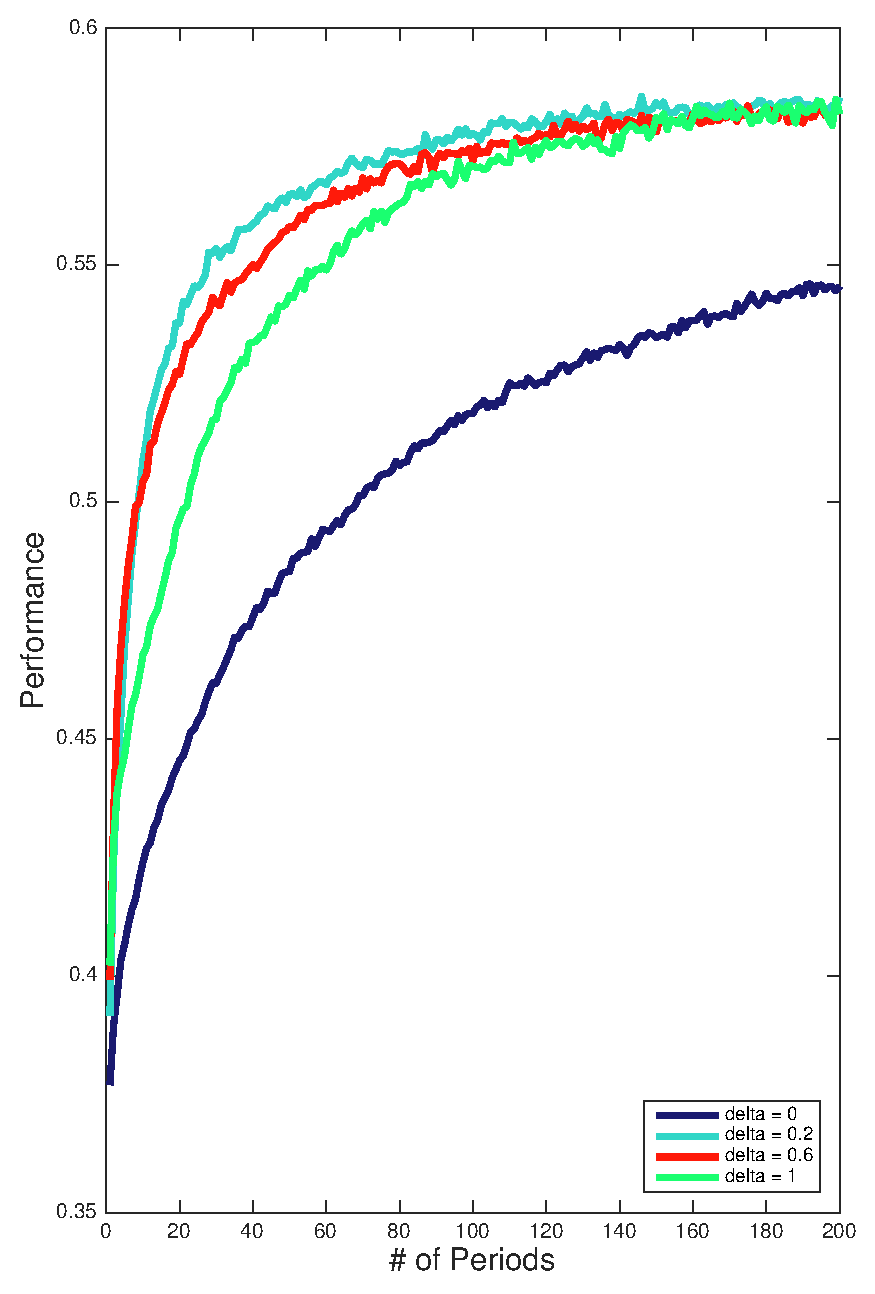
\includegraphics[width=0.45\linewidth]{xpic/adaptordie1.eps} 
	\label{iifig1a050}}
	\quad
	\subfloat[... with highly identical performance landscapes]{%
	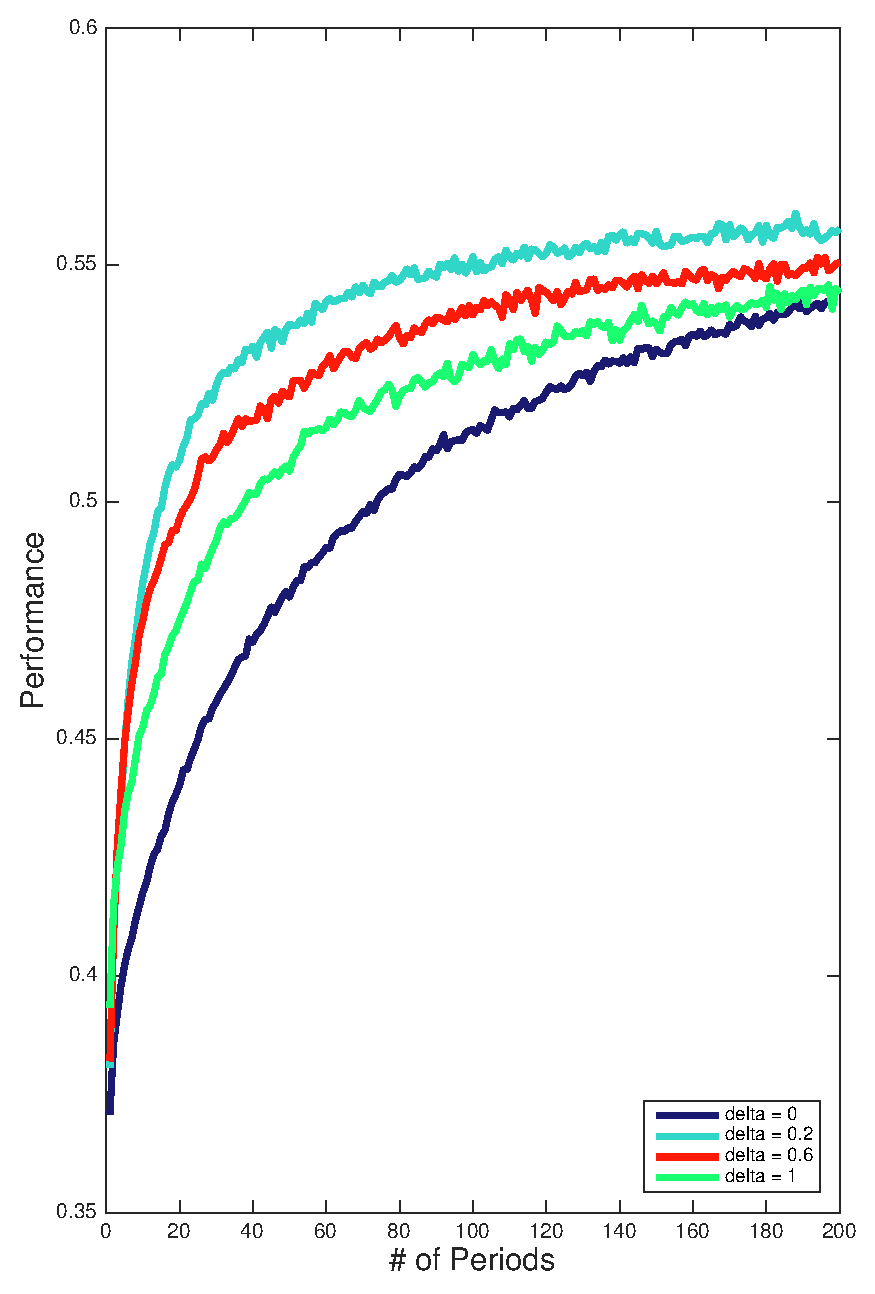
\includegraphics[width=0.45\linewidth]{xpic/adaptordie2.eps}
	\label{ifig1a050}}
	\label{fig:f1}
	\caption{Different learning modes when learning from peers and the performance development over time (with delta indicating the probability of preferring social over individual learning)}
\end{figure}

%\clearpage



\paragraph*{Extension: Learning from organizations that are different. } Figure 2 shows how different learning modes affect performance when learning from other organizations that differs substantially from the own organization. Social learning provides still benefits by improving performance in the short run. However, in the long run (>200 periods), social learning yields lower performance levels than individual learning. The benefits of imitating others by looking at their behavior erodes with increasingly different performance landscapes.


%In figure 2, we compare equilibrium performance at different levels of inter-organizational heterogeneity. Therefore, we take the average performance of organizations that is reached in periods 251-300.\footnote{For these periods, performance levels remain relatively stable and reach their maximum for the conducted simulations.} 
%While equilibrium performance decreases with increasing heterogeneity for updating with complete information (figure 2a), updating with incomplete information yields slightly increasing levels of equilibrium performance with increasing inter-firm heterogeneity (figure 2b). In line with figure 1, selective updating creates higher performance outcomes than unconditional updating for all degrees of heterogeneity.

%This seemingly surprising result can be explained by looking at how the updating mechanisms work: The value of precise updating with complete information about each observed reference erodes with increasing heterogeneity and may even misguide agents in their decisions under settings of high heterogeneity. On the other side, with increasing heterogeneity, Bayesian updating based on incomplete information leads to a less differentiated updating of beliefs. 
%It encourages agents to explore more broadly different alternatives and to experiment even with options that had been less successful at other firms. %The propensity to explore also seemingly less attractive choices becomes increasingly important under higher levels of heterogeneity. %We could observe that steady state performance  with incomplete knowledge increases slightly with an increasing number of firms that can be observed in the ecosystem. 

\begin{figure}[htb]
	\centering
	\subfloat[... with quite different performance landscapes]{%
	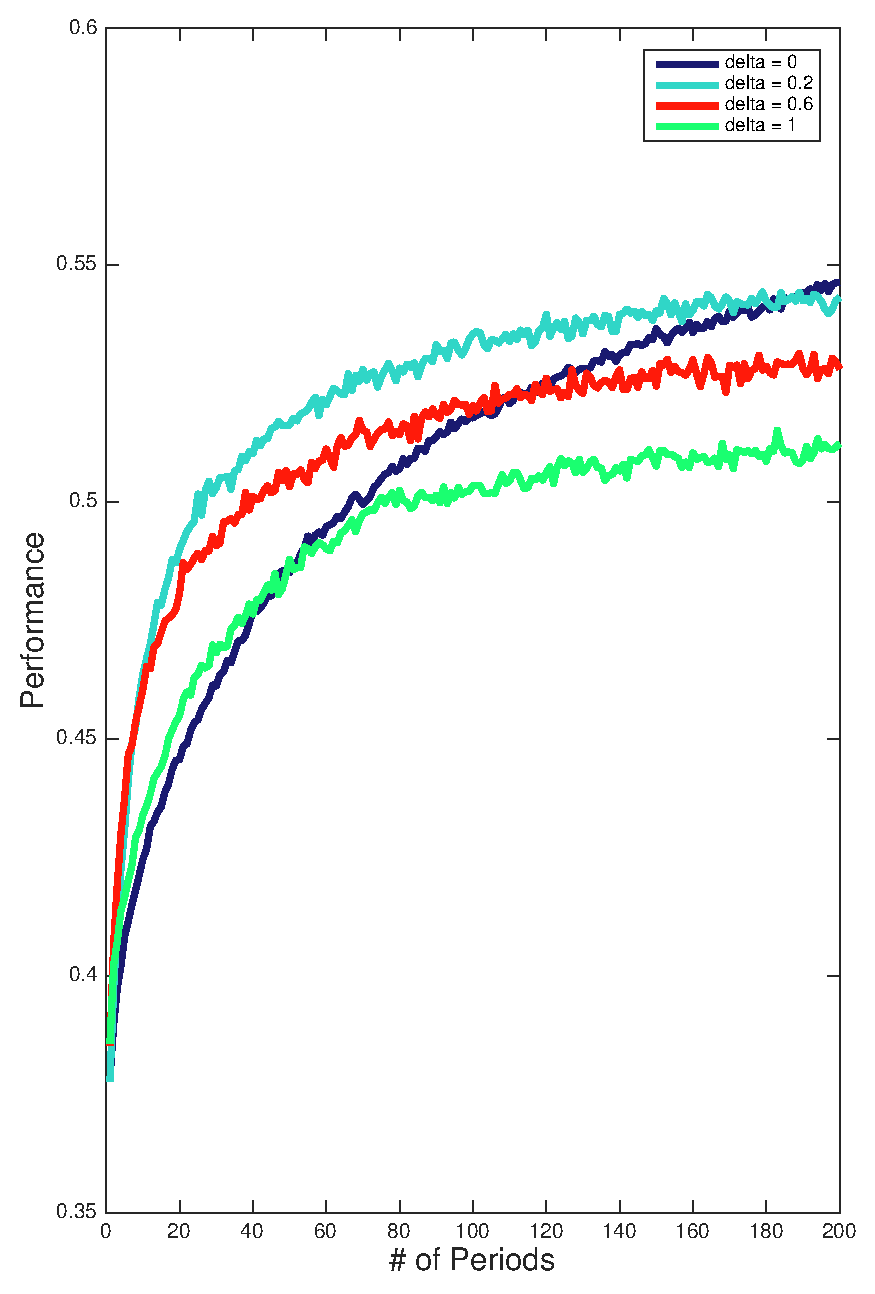
\includegraphics[width=0.45\linewidth]{xpic/adaptordie4.eps} 
	\label{iifig1a050}}
	\quad
	\subfloat[... with very different performance landscapes]{%
	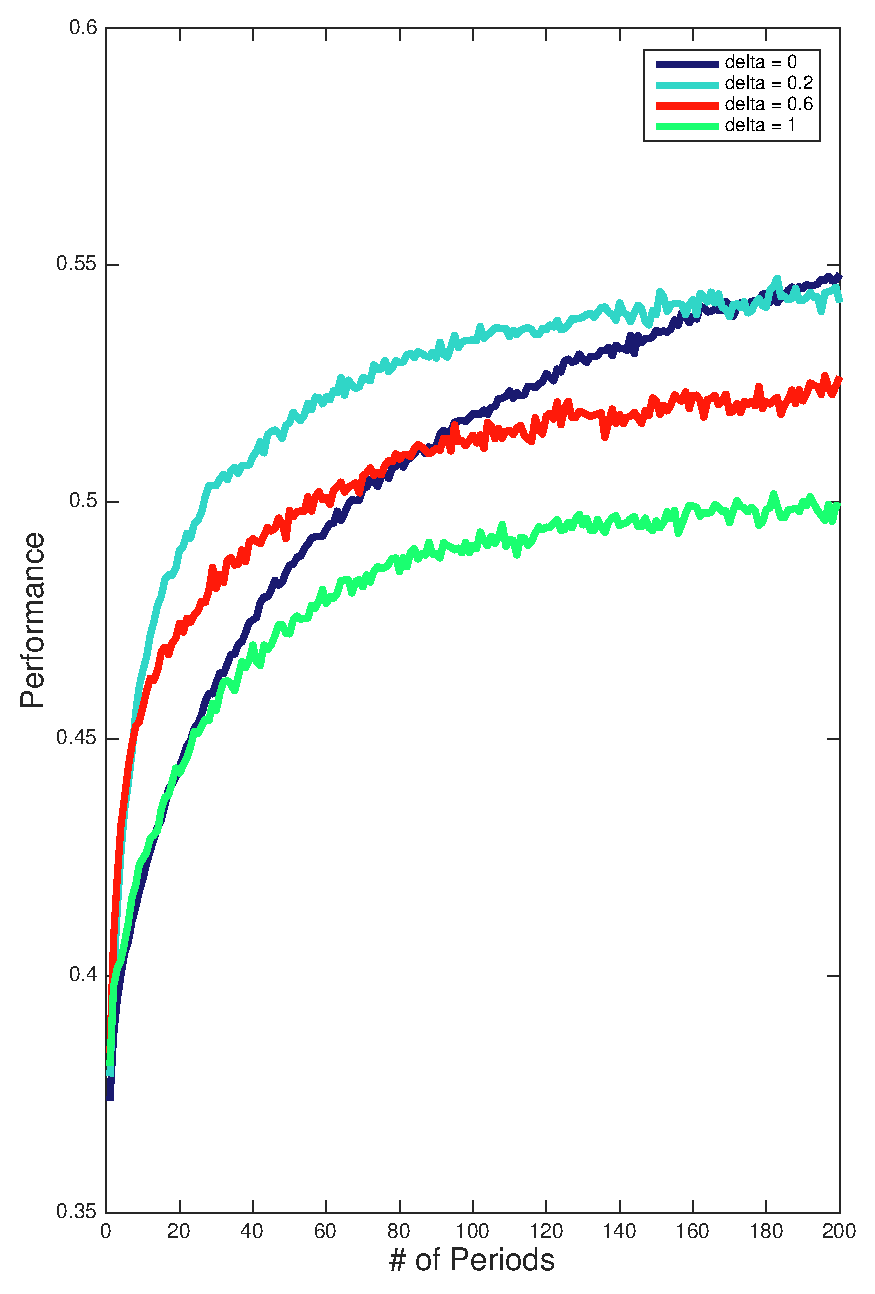
\includegraphics[width=0.45\linewidth]{xpic/adaptordie5.eps}
	\label{ifig1a050}}
	\label{fig:f2}
	\caption{Different learning modes when learning from organizations with different characteristics and the performance development over time (with delta indicating the probability of preferring social over individual learning)}
\end{figure}

%\begin{figure}[htb]
%	\centering
%	\subfloat[Updating using \emph{complete} information]{%
%	\includegraphics[width=0.45\linewidth]{fig4k/iifig2a.eps} 
%	\label{fig2a}}
%	\quad
%	\subfloat[Updating using \emph{incomplete} information]{%
%	\includegraphics[width=0.45\linewidth]{fig4k/ifig2a.eps}
%	\label{fig2b}}
%	\caption{Steady state performance for different degrees of inter-firm heterogeneity}
%	\label{fig:f2}
%\end{figure}
%\clearpage

		
%\subsection*{Experiment 2: Vicarious learning in turbulent times}

%Turbulence is simulated as a shock that occurs with a certain probability at each period and replaces the performance value of each alternative with probability 0.5 (while heterogeneity levels are held constant throughout the simulation).
%With increasing probabilities of turbulence, permanently updating agent's beliefs after each period is the least successful option (figure 3). For the case of complete information, the steady state performance only decreases with higher rates of turbulence for settings of low inter-organizational heterogeneity (figure 3a). For high levels of inter-organizational heterogeneity, steady-state performance remains constant or increases even slightly for increasing probabilities of turbulence (figure 3b). 


%\begin{figure}[htb]
%	\centering
%	\subfloat[Inter-organizational heterogeneity = 0.25]{%
%	\includegraphics[width=0.45\linewidth]{fig4k/jfig3ball_025.eps} 
%	\label{fig3a}}
%	\quad
%	\subfloat[Inter-organizational heterogeneity = 0.75]{%
%	\includegraphics[width=0.45\linewidth]{fig4k/jfig3ball_075.eps}
%	\label{fig3b}}
%	\caption{Steady state performance under varying degrees of turbulence}
%	\label{fig:f3}
%\end{figure}

%\clearpage

%Selective updating prevents agents from too often trying out new approaches when it may make sense to stay with the best or second-best solution of an already known problem of which on average only half of the performance outcomes changed after a turbulence happened. This effect is related to the one observed by \citet{PosenLevinthal2012_Chasing-a-Moving-Target-Exploitation-and-Exploration_MS}, who argue that the acquisition of new knowledge may be eroded too quickly and a renewed focus on exploitation may be  more beneficial. 


\section*{Discussion and Conclusion}

Our results show that information about choices and performance levels which are achieved by other organizations supports the process of (re-)shaping an organization's beliefs and experimentation with choices. Thereby, it stimulates search and helps to overcome structural inertia \citep{hannanfreeman1984}. 
The results of the simulation have the potential to clarify some of the theoretical assumptions of organizational search and explain empirically observed performance differences between firms \citep{audiabrion2007_reluctant-to-change:-self-e, Greve1998_Performance-Aspirations-and-Risky-Organizational_ASQ, ketchen-jr.palmer1999_strategic-responses-to-poor, march1988_variable-risk-preferences-a, March1996_Learning-to-be-Risk-Averse_PsychologicalReview, MarchSimon1958_Organizations,  selten1998_aspiration-adaptation-theor, Singh1986_Performance-Slack-and-Risk-Taking_AMJ, WisemanBromiley1996_Toward-a-Model-of-Risk-in-Declining-Organizations_OS}. The comparison of different degrees of social learning shows that organizations may benefit from combining social search (at moderate levels) with individual search \citep{BinghamDavis2012_Learning-Sequences-Their-Existence-Effect-and-Evolution_AMJ}.

Practitioners need to bear in mind that with increasing heterogeneity within the industry and performance implications that are increasingly dissimilar between organizations, just looking at solutions that worked (on average) best at other companies may be detrimental to improving own firm performance: Under such conditions, the performance may serve as aa benchmark to adjust own aspiration levels, however may not pinpoint the own organization to the respective solution. 
%Setting aspirations and communicating that better performance outcomes should be expected (i.e. are sufficiently likely) is effective -- however artificially narrowing down the search space may decrease the probability that specialists find optimal answers to reoccurring challenges. 


\clearpage
% -----------------------------------------------------------------------------------------------------------------------
% Appendix 
% -----------------------------------------------------------------------------------------------------------------------
	\newpage
	\begin{appendix}
	\setstretch{1.05}
	\scriptsize
	%	\begin{multicols}{2}
			\renewcommand*{\bibfont}{\footnotesize}
			\printbibliography
	%	\end{multicols}				

%%\newpage
%%\section*{Add-ons}
%%
%%\begin{compactitem}[$\circ$]
%%	\item limited rationality and ambiguity in organizational learning \cite{MarchOlsen1975_The-Uncertainty-of-the-Past-Organizational-Learning_EJoPR}
%%	\item learning from failure \citep{KimMiner2007_Vicarious-Learning-From-the-Failures-and-Near}
%%	\item Aspiration levels are influenced both internally, such as through an organization's history of past performance, and externally, such as through reference organizations \citep{Greve1998_Performance-Aspirations-and-Risky-Organizational_ASQ, HsiehTsai2014_If-they-can-do-it-why-not-us-Competitors-as-r,BlettnerHe2014_Adaptive-aspirations-and-performance-heterogeneity_SMJ}.
%%	\item External benchmarking and setting aspirations based on other organizations' performance may go even beyond performance improvement and be an important source of innovation: \citet{AntonelliScellato2013_Complexity-and-technological-change-knowledge-interactions_JoEE} find that interorganizational interactions are important to generate new technological knowledge. They see innovation as something that emerges from a system rather than single firms. 
%%	\item \cite{SrinivasanHaunschild2007_Vicarious-Learning-in-New-Product-Introduction_MS}
%%	\item Thereby, we look at how knowledge evolves in an interconnected system when different sources, and especially external sources of information are combined. Thereby this simulation is distinct from other studies, such as \citet{PosenMartignoni2013_Rubiks-Dilemma-Partial-Knowledge-and-the-Effect-of-Learning_AoMP}, who look at how prior knowledge influences subsequent search.
%%\end{compactitem}
%%
%%\citet{KnudsenSrikanth2014_Coordinated-Exploration-Joint-Search_ASQ} state that hierarchy cannot improve search mechanisms and how problems should be addressed (unless the superior has perfect knowledge about possible performance outcomes). We disagree with this statement and interpret hierarchy differently. 
%%We investigate a mechanism under which hierarchy can improve joint organizational search (despite the superior is missing perfect information about all possible outcomes and combinations as stated by them):
%%If a superior is able to compare the own organization's performance with the performance of related organizations that are facing similar problems, such a comparison may serve as an additional, valuable reference. Such external observations can increase performance if brought inside the organization and leveraged to alter beliefs, which then direct search efforts by updating the specialist's beliefs about how to solve a given problem.
%%% The impact of selective organizational attention and feedback bears still great potentials for future research \citep{KeilLang2014_Is-Selective-Attention-Always-Beneficial_AoMP}. 
%%
%%
%%
%%
%%\citep{TerlaakGong2008_Vicarious-Learning-and-Inferential-Accuracy-i}. 
%%
%%
%%
%%* Organizational learning may not always be beneficial: Superstitious learning \citep{Zollo2009_Superstitious-Learning-with-Rare-Strategic-Decisions_OS}
%%
%%
%%\noindent \hrulefill
%%
%%Such learning may also happen by learning from others, such as in partnerships and strategic alliances -- but also by learning from competitors or other organizations. 
%%
%%Observing other organizations if dealing with related problems is always a benchmark/ orientation. Organizational performances compared to the performance of competitors. Seeing other organizations performing better (or worse) may then influence an organization's own expectations and aspiration levels. We distinguish two different settings: 
%%\begin{compactenum}
%%	\item Organizations may directly learn from others: \newline If an organization sees how a problem is addressed and what the performance outcomes are, such observations may impact internal search ($\rightarrow$ stimulating exploration into a certain direction)
%%	\item Often however, only performance can be observed -- organizations see that better performance should be possible, however, they can't observe how this can be achieved. Thereby, watching others has an effect that $\rightarrow$ stimulates exploration without directing it. 
%%\end{compactenum}
%%
%%\noindent \hrulefill
%%
%%
%%The multi-armed bandit is one of the canonical simulation models used to analyze (organizational) learning. Over multiple periods, an agent has the choice between $N$ decision alternatives, with each decision implying different payoff amounts and probabilities, which are initially unknown. Thus, the agent has to balance the activities of (a)  \emph{exploring} in order to advance his knowledge about the payoff distributions and (b) \emph{exploiting} existing knowledge in order to maximize payoffs over the remaining periods \citep{March1991_Exploration-and-Exploitation_OS}.%
%%% The multi-armed bandit model is used in various fields and has many theoretical and practical applications. 
%%\footnote{The idea of extending the classic armed bandit model to a setting of multiple agents that all face the same optimization problem is not completely new. \citet{BoltonHarris1999_Strategic-Experimentation_Econometrica} use a two-armed bandit problem to analyze how learning changes if agents can directly learn from the experimentation of other agents. However, their underlying model assumes (full/perfect) information as a publicly available good and doesn't incorporate heterogeneity between agents. Thus, the here analyzed problem is related, however our investigated effects differ substantially from the aforementioned research.}
%%
%%% We look here at a different problem: Assuming that the generalist and the specialist are willing to cooperate and optimally work together, we investigate how arising organizational challenges are best addressed by optimally using the knowledge/resources of both parties.
%%
%%Our organization consists of a two individuals, a lower-level decision maker, called the agent, who addresses the problem and one superior, called the principal who is informing the agent about expected outcomes and actions in comparison with related organizations. 
%%
%%We distinguish between a principal who only has 
%%(i) incomplete knowledge (i.e.\;only observes the performance, but not the choice of other organizations dealing with a specific problem) and a principal who has 
%%(ii) complete knowledge about the responses of the other organizations (i.e.\;can see both the performance \emph{and} the chosen approach to address a specific problem).
%%We analyze how different rates of firm heterogeneity (i.e.\;differences between the performance outcomes of available choices to address a problem) and different levels of change (i.e.\;different rates at which performance outcomes of the available response options change) affect organizational performance.
%%
%%At it's core, the multi-armed bandit model is about the process of search for the optimal solution and balancing  between experimental exploration of unknown alternatives and exploiting alternatives that have been tried out before \citep{DenrellMarch2001_Adaptation-as-Information-Restriction-The-Hot-Stove_OS}. 
%%
%%
%%
%%Our simulations confirm that the knowledge of how other organizations address similar problems can be leveraged to increase performance. In general, the higher the similarity of the problems solved by the observed firms, the better complete knowledge about the other firms' approaches to solve the problems can be used to increase one's own performance. With increasing heterogeneity (i.e. optimal solutions to problems differ between firms with increasing probabilities), the less valuable accurate information about how other firms address the same problems becomes. Surprisingly, under conditions of high inter-firm heterogeneity, less accurate information that only includes other firm's payoffs, however not their solution approaches, may be even more valuable to inform/update intra-firm beliefs and guide search in subsequent periods. 
%%Thereby, we contradict the classic/established assumptions that a firms' knowledge about it's strategic options (and their expected payoffs) has an (unconditional) positive effect on performance
%%\citep{Grant1996_Toward-a-Knowledge-Based-Theory-of-the-Firm_SMJ, KogutZander1992_Knowledge-of-the-Firm-Combinative-Capabilities_OS, Porter1985_How-information-gives-you-competitive-advantage_HBR, ZanderKogut1995_Knowledge-and-the-Speed-of-the-Transfer_OS}.
%%We contribute to the understanding of how organizations learn by combining internal search with the observation of how other organizations address similar problems. 
%%
%%Further, it prevents firms from getting stuck at sub-optimal solutions. Related, but differently from competency traps \citep{LevinthalMarch1993_The-myopia-of-learning_SMJ, Levinthal1997_Adaptation-on-rugged-landscapes_MS}, performance levels of other organizations serve as references and avoid the tendency of suppressing exploration and favoring already known, sub-optimal solutions. 
%%	
%%Empirical research has shown that explorative activities that aim at improving an organization's long-term performance may depend on an organization's relative performance within the industry. Organizations performing below aspirations often behave inconsistently with regard to experimental search activities and past findings have been partly contradicting. 	
%%	
%%
%%
%%Further, we show that a principal's incomplete information may be sufficient to guide search and substantially improve performance. Thereby, we contradict \citet{KnudsenSrikanth2014_Coordinated-Exploration-Joint-Search_ASQ} who argue that hierarchy needs to be informed in advance with perfect information in advance about the global peak in order to have a positive impact on organizational search. We further contradict established assumptions \citep{Grant1996_Toward-a-Knowledge-Based-Theory-of-the-Firm_SMJ, KogutZander1992_Knowledge-of-the-Firm-Combinative-Capabilities_OS, Porter1985_How-information-gives-you-competitive-advantage_HBR, ZanderKogut1995_Knowledge-and-the-Speed-of-the-Transfer_OS} by finding that more accurate knowledge about others is may not be always beneficial for imitation \citep{Rivkin2000_Imitation-of-Complex-Strategies_MS}.
%%
%%Further, the analysis shows that a \emph{knolwedge-integration capability} to translate various sources of information optimally into performance is important \citep{GardnerStaats2012_Dynamically-Integrating-Knowledge-in-Teams_AMJ}.
%%
%%
%%The simulations show that knowledge about both performance outcomes and choices made by other organizations is valuable to stimulate and direct search. However, Managers 	
%%	
%%Often, it is implicitly assumed that exploration and discovering a good or optimal solution is the problem -- however, this simulation uncovers that it may be rather misaligned aspiration levels that prevent organizations from investing in exploration. Benchmarking with related organizations may be effective to overcome this trap of under-exploring, even if observations are not fully accurate and managers only gain incomplete knowledge from competitors. 
%%	
	
	\end{appendix}
\end{document}

%%-------------------------------
%


% -----------------------------------------------------------------------------------------------------------------------
% all this: already in TXT-document
% -----------------------------------------------------------------------------------------------------------------------
%
%% -----------------------------------------------------------------------------------------------------------------
%% Text  - Appendix 
%% -----------------------------------------------------------------------------------------------------------------
%\appendix
%% \newpage
%% \pagenumbering{Roman} 
%\footnotesize
%\begin{appendix}
%
%\nopagebreak
%\twocolumn
%
%\printbibliography
%			
%\end{appendix}
%\end{document}